%
% This is the LaTeX template file for lecture notes for CS294-8,
% Computational Biology for Computer Scientists.  When preparing 
% LaTeX notes for this class, please use this template.
%
% To familiarize yourself with this template, the body contains
% some examples of its use.  Look them over.  Then you can
% run LaTeX on this file.  After you have LaTeXed this file then
% you can look over the result either by printing it out with
% dvips or using xdvi.
%
% This template is based on the template for Prof. Sinclair's CS 270.

\documentclass{article}
\usepackage{graphics}
\usepackage{multicol}
\usepackage{tikz}
\usepackage{clrscode3e}
\usepackage{enumitem}
\usepackage{amsmath}
\usepackage{amsthm}
\usepackage{amssymb}

\setlength{\oddsidemargin}{0 in}
\setlength{\evensidemargin}{0 in}
\setlength{\topmargin}{-0.6 in}
\setlength{\textwidth}{6.5 in}
\setlength{\textheight}{8.5 in}
\setlength{\headsep}{0.75 in}
\setlength{\parindent}{0 in}
\setlength{\parskip}{0.1 in}

%
% The following commands set up the lecnum (lecture number)
% counter and make various numbering schemes work relative
% to the lecture number.
%
\newcounter{lecnum}
\renewcommand{\thepage}{\thelecnum-\arabic{page}}
\renewcommand{\thesection}{\thelecnum.\arabic{section}}
\renewcommand{\theequation}{\thelecnum.\arabic{equation}}
\renewcommand{\thefigure}{\thelecnum.\arabic{figure}}
\renewcommand{\thetable}{\thelecnum.\arabic{table}}

%
% The following macro is used to generate the header.
%
\newcommand{\lecture}[4]{
   \pagestyle{myheadings}
   \thispagestyle{plain}
   \newpage
   \setcounter{lecnum}{#1}
   \setcounter{page}{1}
   \noindent
   \begin{center}
   \framebox{
      \vbox{\vspace{2mm}
    \hbox to 6.28in { {\bf CSC2420 - Algorithm Design, Analysis and Theory
                        \hfill Fall 2022} }
       \vspace{4mm}
       \hbox to 6.28in { {\Large \hfill Lecture #1: #2  \hfill} }
       \vspace{2mm}
       \hbox to 6.28in { {\it Lecturer: #3 \hfill Scribe: #4} }
      \vspace{2mm}}
   }
   \end{center}
   \markboth{Lecture #1: #2}{Lecture #1: #2}
   % {\bf Disclaimer}: {\it These notes have not been subjected to the
   % usual scrutiny reserved for formal publications.  They may be distributed
   % outside this class only with the permission of the Instructor.}
   \vspace*{4mm}
}

%
% Convention for citations is authors' initials followed by the year.
% For example, to cite a paper by Leighton and Maggs you would type
% \cite{LM89}, and to cite a paper by Strassen you would type \cite{S69}.
% (To avoid bibliography problems, for now we redefine the \cite command.)
% Also commands that create a suitable format for the reference list.
\renewcommand{\cite}[1]{[#1]}
\def\beginrefs{\begin{list}%
        {[\arabic{equation}]}{\usecounter{equation}
         \setlength{\leftmargin}{2.0truecm}\setlength{\labelsep}{0.4truecm}%
         \setlength{\labelwidth}{1.6truecm}}}
\def\endrefs{\end{list}}
\def\bibentry#1{\item[\hbox{[#1]}]}

%Use this command for a figure; it puts a figure in wherever you want it.
%usage: \fig{NUMBER}{SPACE-IN-INCHES}{CAPTION}
\newcommand{\fig}[3]{
			\vspace{#2}
			\begin{center}
			Figure \thelecnum.#1:~#3
			\end{center}
	}
% Use these for theorems, lemmas, proofs, etc.
\newtheorem{theorem}{Theorem}[lecnum]
\newtheorem{lemma}[theorem]{Lemma}
\newtheorem{proposition}[theorem]{Proposition}
\newtheorem{claim}[theorem]{Claim}
\newtheorem{corollary}[theorem]{Corollary}
\newtheorem{definition}[theorem]{Definition}
\newtheorem{problem}[theorem]{Problem}
\newtheorem{conjecture}[theorem]{Conjecture}
\renewenvironment{proof}{{\bf Proof:}}{\hfill\rule{2mm}{2mm}}

\newcommand{\Exp}{\mathbb{E}}
\newcommand{\Var}{\mathrm{Var}}

\usepackage{vwcol}

\begin{document}
%FILL IN THE RIGHT INFO.
%\lecture{**LECTURE-NUMBER**}{**DATE**}{**LECTURER**}{**SCRIBE**}
\lecture{5}{Matroid, Local Search}{Allan Borodin}{Kevin Gao}

\section{Set Packing}

We will consider the $s$-set packing problem and two greedy algorithms: one relatively ``natural'' greedy algorithm, and one that is not so natural.

\begin{problem}
    We are given $n$ subsets $S_1,\ldots,S_n$ from a universe $U$ of size $m$. In the weighted case, each subset $S_i$ has a weight $w_i$. The goal is to choose a disjoint subcollection $\mathcal{S}$ of the subsets so as to maximize $\sum_{S_i \in \mathcal{S}} w_i$. In the $s$-set packing problem, we have $|S_i| \leq s$ for all $i$.
\end{problem}

By reduction from max-clique, there is an $m^{1/2 - \epsilon}$ hardness of approximation result assuming NP $\neq$ ZPP. For $s$-set packing with constant $s \geq 3$, there is an $\Omega(s / \log s)$ hardness of approximation assuming P $\neq$ NP.

\subsection{Greedy by Weight}

\begin{codebox}
    \Procname{$\proc{Greedy-By-Weight}$}
    \li sort the sets so that $w_1 \geq w_2 \geq \ldots \geq w_n$
    \li $\mathcal{S} = \emptyset$
    \li \For $i = 1$ \To $n$ \Do
        \li \If $S_i$ does not intersect any set in $\mathcal{S}$ \Then
            \li $\mathcal{S} = \mathcal{S} \cup \{S_i\}$  
\end{codebox}

\begin{theorem} \label{thm:set-packing-ratio}
    \proc{Greedy-By-Weight} provides an $s$-approximation for the $s$-set packing problem.
\end{theorem}

\begin{proof}
    \begin{vwcol}[widths={0.7,0.3},sep=.8cm, justify=flush,rule=0pt,indent=1em]
        We prove this using a charging argument. It suffices to show a charging function $\chi:\; OPT \to ALG$ such that for any set $S_j \in ALG$, the weight of sets in $OPT$ charged to $S_j$ is at most $s \cdot w_j$. We charge the weight of every set in $OPT$ to the first set in the greedy solution with which it intersects. Such set must exist in $ALG$ because otherwise if some set in $OPT$ does not intersect with any sets in $ALG$, it can just be taken by $ALG$ as part of the solution entirely. Since $|S_j| \geq s$, at most $s$ sets in $OPT$ can be charged to the same $S_j$. If $S_i^*$ is charged to $S_j$, then $w_i \leq w_j$ because otherwise greedy would have taken $S_i^*$ instead.
        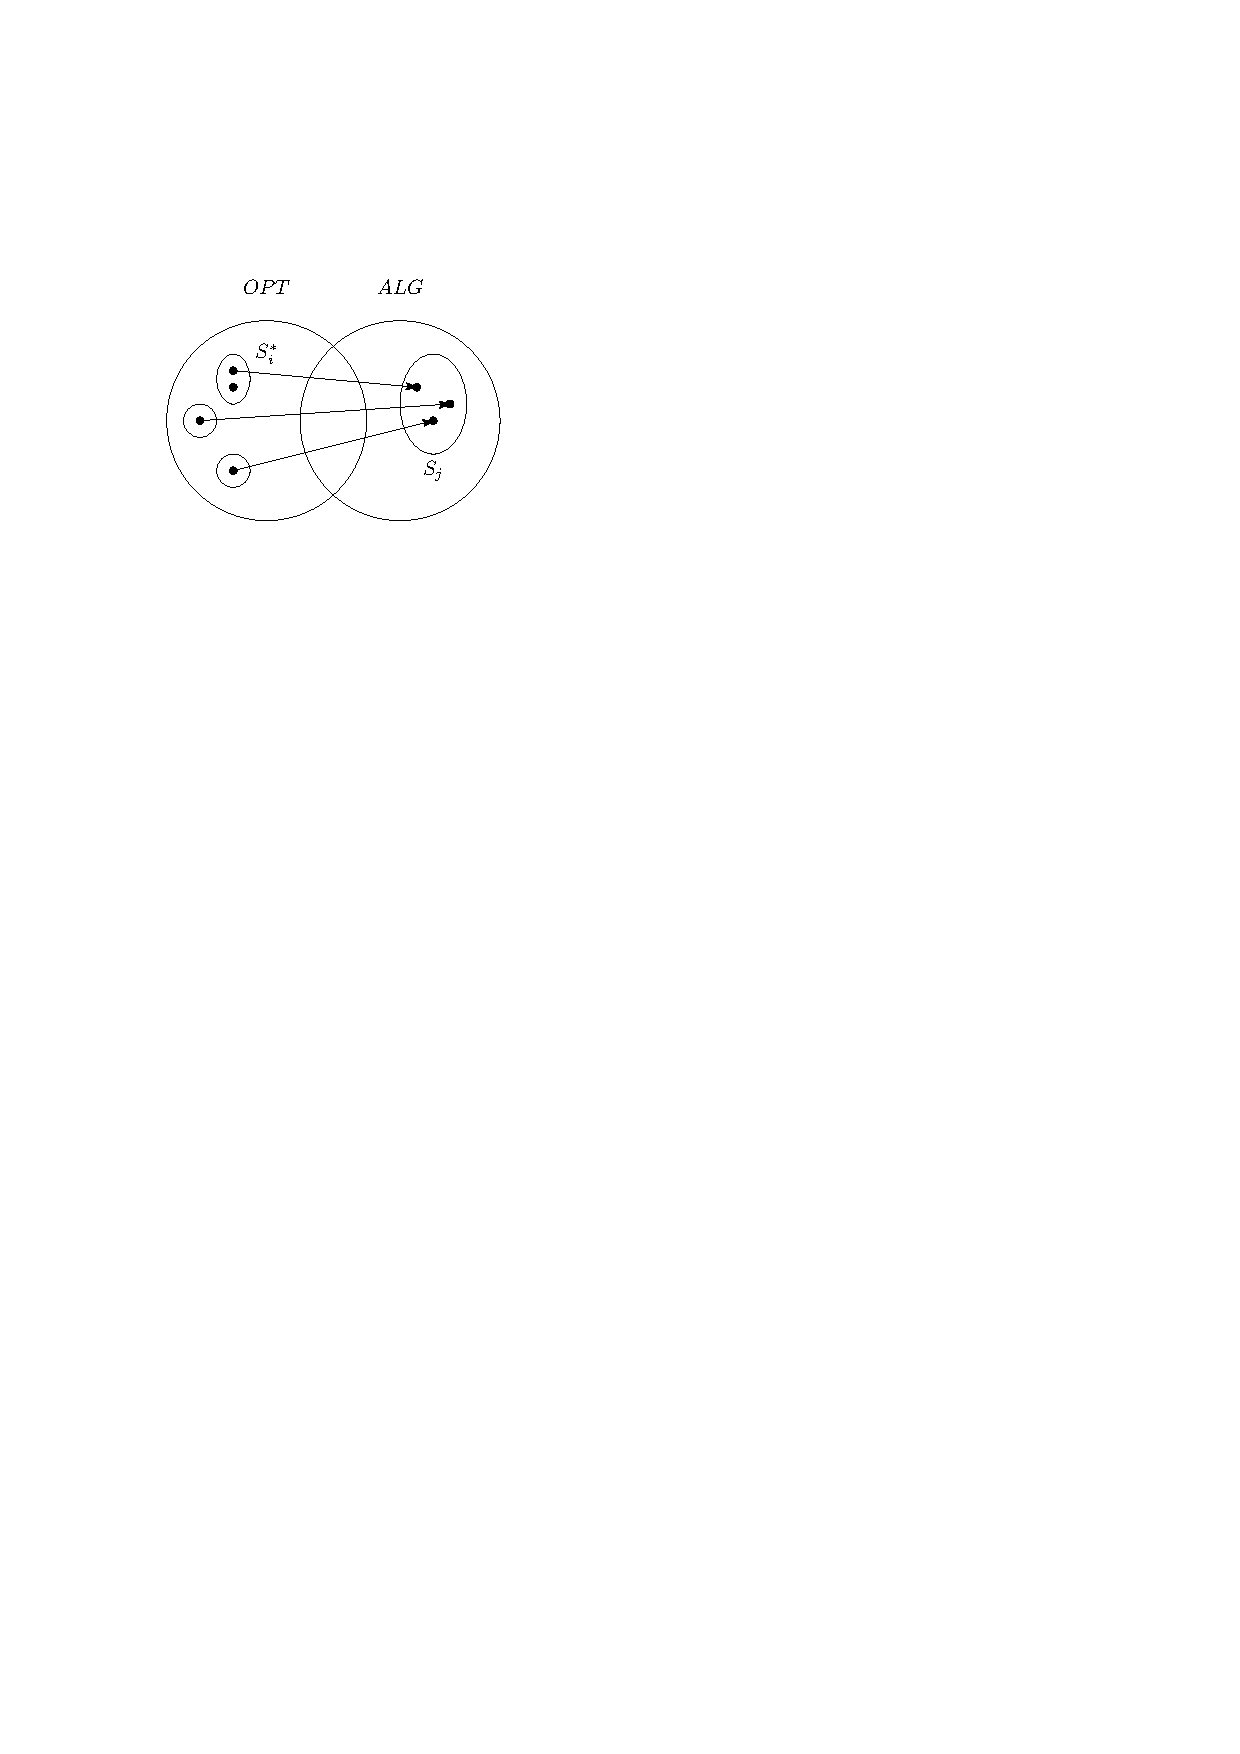
\includegraphics[width=0.25\linewidth]{set-cover-charging-argument.pdf}
    \end{vwcol}
\end{proof}

\subsection{Charging Argument}

The argument that we used for Theorem \ref{thm:set-packing-ratio} is known as the charging argument. It can be used to show both the correctness (optimality) of greedy algorithms and the approximation ratio. To show some algorithm obtains the globally optimal solution of some maximization problem, one needs to show that the algorithm produces an output with as much ``profit'' as the optimal solution. It suffices to find a 1-to-1 function $f:\; OPT \to ALG$. By providing such a function and showing that it is 1-to-1, we would have $|OPT| \leq |ALG|$, which proves the optimality of the algorithm. Similarly, for minimization problem, it suffices to give a 1-to-1 function $h:\; ALG \to OPT$ which would imply $|ALG| \leq |OPT|$.

The same argument can be used to prove approximation ratios. For maximization problem, we charge (map) the profit of some optimal solution $OPT$ to the profit of $ALG$. We can then argue that not too much profit from $OPT$ gets charged (mapped) to $ALG$. For this, it suffices to prove that the charging function is $\epsilon$-to-1 where $\epsilon$ is the desired approximation ratio.

\subsection{Greedy by Weight per Square Root of Size}

If all sets have unit weight, greedy by weight-per-size is known to provide a $\sqrt{s}$-approximation, but this is just the same as ordering the input sets so that $|S_1| \leq |S_2| \leq \ldots \leq |S_n|$. However, greedy by weight-per-size does not improve the $s$ approximation ratio for the weighted case. One heuristic that improves the approximation ratio is to instead order the sets by their weight-per-square root of size.

\begin{codebox}
    \Procname{$\proc{Greedy-By-Weight-Per-Sqrt-Size}$}
    \li sort the sets so that $\frac{w_1}{\sqrt{|S_1|}} \geq \frac{w_2}{\sqrt{|S_2}} \geq \ldots \geq \frac{w_n}{\sqrt{|S_n|}}$
    \li $\mathcal{S} = \emptyset$
    \li \For $i = 1$ \To $n$ \Do
        \li \If $S_i$ does not intersect any set in $\mathcal{S}$ \Then
            \li $\mathcal{S} = \mathcal{S} \cup \{S_i\}$  
\end{codebox}

\begin{theorem}
    \proc{Greedy-By-Weight-Per-Sqrt-Size} provides a $2 \sqrt{m}$-approximation for the set packing algorithm. We note that $\sqrt{m}$ is asymptotically the best possible approximation assuming NP $\neq$ ZPP.
\end{theorem}

\subsection{Partial Enumeration Greedy}

Alternatively, one can use the partial enumeration greedy approach for the set packing problem. The algorithm \proc{Partial-Greedy} is described as follows. Let $\mathrm{MAX}_k$ be the optimal solution of the set packing problem restricted to those containing at most $k$ sets. Let $G$ be the solution by \proc{Greedy-By-Weight} restricted to the sets of cardinality of at most $\sqrt{m/k}$. Return the best of $\mathrm{MAX}_k$ and $G$.

\begin{theorem}
    \proc{Partial-Greedy} achieves a $2\sqrt{m/k}$ approximation for the weighted set packing problem on a universe of size $m$.
\end{theorem}


\section{Matroids}

\begin{definition}[Matroid]
    Let $U$ be a set of elements and $\mathcal{I}$ be a collection of subsets of $U$. $(U,\mathcal{I})$ is a \textbf{matroid} if the following holds:
    \begin{itemize}
        \item heraitary property: if $I \in \mathcal{I}$ and $I' \subset I$, then $I' \in \mathcal{I}$
        \item exchange property: if $I',I \in \mathcal{I}$ and $|I'| < |I|$, then $\exists u \in I \setminus I'.\, I' \cup \{u\} \in \mathcal{I}$  
    \end{itemize}
\end{definition}

An \textbf{hereditary set system} $(U,\mathcal{I})$ is any set system satisfying the hereditary property so that a matroid is a hereditary set system that also satisfies the exchange property. The sets $I \in \mathcal{I}$ are called the \textbf{independent sets}. The \textbf{maximal independent set} of a matroid is also referred to as the \textbf{bases} of the matroid. By the exchange property, all maximal independent sets of a given matroid have the same cardinality, known as the \textbf{rank} of the matroid. Many of the terminologies used for matroid are similar to those in linear algebra. This is best illustrated with a \textbf{graph matroid} and the corresponding \textbf{vector matroid} induced by the graph.

Alternatively, a matroid can be defined in terms of \textbf{circuits}.

\begin{definition}[Alternative Definition of Matriod]
    Let $U$ be a set of elements and $\mathcal{C}$ be a collection of subsets of $U$. $(U,\mathcal{C})$ is a matroid if
    \begin{itemize}
        \item If $C_1,C_2 \in \mathcal{C}$ and $C_1 \subseteq C_2$, then $C_1 = C_2$
        \item If $C_1$ and $C_2$ are distinct members of $\mathcal{C}$ and $e \in C_1 \cap C_2$, then $\mathcal{C}$ contains some $C_3$ such that $C_3 \subseteq (C_1 \cup C_2) \setminus \{e\}$.
    \end{itemize}
\end{definition}

The objective of max weighted independent set in a matroid is to select an independent set $I \subseteq U$ that maximizes $\sum_{u \in I} w(u)$ where $w(u)$ is the weight of element $u$. 

Kruskal's algorithm for MST can be thought as the max weighted independent set problem on a graph matroid. For example, an independent set of vectors in a vector space is a matroid (Whitney 1935).

A standard greedy algorithm for a max independent set.

\begin{codebox}
    \li $\mathcal{S} = \emptyset$
    \li \While $\exists u.\, \mathcal{S} \cup \{u\}$ is independent \Do
        \li $\mathcal{S} = \mathcal{S} \cup \{u\}$ where $u$ is an element of largest weight such that $\mathcal{S} \cup \{u\}$ is independent
\end{codebox}

\begin{theorem}[Rados]
    For independence in a matroid $M$, Greedy is an optimal algorithm for maximizing the weight of basis (i.e. maximizing a linear function subject to a matroid constraint).
\end{theorem}

\begin{theorem}[Edmonds]
    Consider any hereditary set system. If the natural greedy algorithm produces an optimal solution for every linear function of elements in an independent set, then the set system is a greedy algorithm.
\end{theorem}

Does matroid formalizes greedy algorithms? No, it does not say anything about approximation algorithms.

Is the optimality of greedy algorithms limited to independent sets in matroids? No. Consider the greedy algorithm for unweighted interval scheduling on $m$ identical machines, which does not satisfy the exchange property.

\section{Local Search}

Along with greedy and greedy-like algorithms, local search is one of the two conceptually simplest optimization paradigms.

\begin{codebox}
    \li initialize $S$ 
    \li \While there is a better solution $S'$ in the local nbhd of $S$ \Do
        \li $S = S'$
    \End
\end{codebox}

If and when the algorithm terminates, the algorithm has computed a local optimum. However, some key problems remain:

\begin{itemize}
    \item How are we allowed to choose an initial solution?
    \item What constitutes a reasonable definition of a ``local neighborhood''?
    \item What do we mean by ``better''?
\end{itemize}

For some applications, it turns out that rather than searching to improve the given objective function, we search for a solution in the local neighborhood that improves a related \textbf{potential function} and this has been termed \textbf{non-oblivious local search}.

\subsection{Oblivious Local Search for Exact Max-2-SAT}

Recall the Max-$k$-SAT problem. We are given a CNF formula with $k$ variables. We would like to find a truth assignment that maximizes the number of satisfied clauses. In the weighted case, we want to instead maximize the combined weight of the satisfied clauses. The unweighted case is simply the weighted case with the weight of each clause set to 1.

\begin{codebox}
    \Procname{$\proc{Max-2-SAT-Local-Search}$}
    \li $\tau = $ any initial truth assignment
    \li \While $\exists \hat{\tau} \in N_d(\tau),\, W(\hat{\tau}) > W(\tau)$ \Do
        \li $\tau = \hat{\tau}$
    \End
\end{codebox}
where $N_d(\tau)$ represents the $d$-neighborhood of $\tau$ defined to be $\{\tau' \mid \text{$\tau$ and $\tau'$ differ on at most $d$ variables}\}$.


\begin{theorem}
    The approximation ratio for \proc{Max-2-SAT-Local-Search} is $2/3$.
\end{theorem}

\begin{proof}
    Let $\tau$ be a local optimum and let
    \begin{itemize}
        \item $S_0$ be the set of clauses not satisfied by $\tau$
        \item $S_1$ be the set of clauses satisfied with exactly one literal by $\tau$
        \item $S_2$ be the set of clauses satisfied with two literals by $\tau$ 
    \end{itemize}
    Let $W(S_i)$ be the corresponding weight. We say a clause involves a variable $x_j$ if either $x_j$ or $\neg x_j$ occurs in the clause. Then, for each $j$, let

    \begin{itemize}
        \item $A_j$ be those clauses in $S_0$ involving the variable $x_j$.
        \item $B_j$ be those clauses $C$ in $S_1$ involving the variable $x_j$ such that it is the literal $x_j$ or $\neg x_j$ that is satisfied in $C$ by $\tau$.
        \item $C_j$ be those clauses in $S_2$ involving $x_j$.
    \end{itemize}
    Similarly, let $W(A_j),W(B_j),W(C_j)$ be the corresponding weights. Summing the weights over all variables, we get
    $$
    2W(S_0) = \sum_{j} W(A_j)
    $$
    becuase each clause in $S_0$ gets counted twice when we sum over the variables. For $S_1$, we have
    $$
    W(S_1) = \sum_{j} W(B_j).
    $$
    Given that $\tau$ is a local optimum, for every $j$, we have
    $$
    W(A_j) \leq W(B_j)
    $$
    or else flipping the truth value of $x_j$ would improve the weight of the clauses being satisfied. Hence, by summing over all $j$, we have $2W_0 \leq W_1$. It follows that the ratio of clause weights not satisfied to the numb of all clause weights is
    $$
    \frac{W(S_0)}{W(S_0)+W(S_1)+W(S_2)} \leq \frac{W(S_0)}{3W(S_0)+W(S_2)} \leq \frac{W(S_0)}{3W(S_0)}.
    $$
\end{proof}

From the analysis of the approximation ratio of the oblivious local search algorithm, we can gain some knowledge as to how to improve the algorithm. Note that we are not using anything about $W(S_2)$ in the analysis. If we could guarantee that $W(S_0)$ was at most $W(S_2)$, then the ratio of clause weights not satisfied to all clause weights would be $1/4$. The idea of the improved non-oblivious local search algorithm is to weigh $S_2$ clauses more heavily. Intuitively, the $S_2$ clauses are more valuable since they are more ``resilient'' to any single variable change.

Specifically, in the improved algorithm for Max-2-SAT, in each iteration where we find $\tau' \in N_1(\tau)$, we take the one that improves the \textbf{potential function}
$$
\frac{3}{2} W(S_1) + 2W(S_2)
$$
instead of $W(S_1) + W(S_2)$.

More generally, for Max-$k$-SAT, we set a set of scaling coefficients $c_1,\ldots,c_k$ such that the non-oblivious local search optimizes the potential function
$$
c_1W(S_1) + c_2W(S_2) + \cdots + c_k W(S_k).
$$
This gives an approximation ratio of $\frac{2^k - 1}{2^k}$ for exact Max-$k$-SAT.

Next, we will sketch a proof for the $3/4$ approximation ratio for the non-oblivious local search algorithm for Max-2-SAT.

\begin{theorem}
    \proc{Non-Oblivious-Max-2-SAT} achieves an approximation ratio of $3/4$.
\end{theorem}

\begin{proof}
    Without loss of generality, we assume that $\tau$ is the all-true assignment. Let $P_{i,j}$ be the weight of all clauses in $S_i$ containing $x_j$. Let $N_{i,j}$ be the weight of all clauses in $S_i$ containing $\neg x_j$. For some local optimum $\hat{\tau}$ with respect to the potential function $3/2 W(S_1) + 2W(S_2)$, for all variables $x_j$,
    $$
    -\frac{1}{2} P_{2,j} - \frac{3}{2} P_{1,j} + \frac{1}{2} N_{1,j} + \frac{3}{2} N_{0,j} \leq 0.
    $$
    Summing over all variables, $P_1 = N_1 = W(S_1)$ and $P_2 = 2W(S_2)$ and $N_0 = 2W(S_0)$. It follows from the above inequality that
    $$
    3W(S_0) \leq W(S_1) + W(S_2).
    $$
\end{proof}

\end{document}